
\chapter{Mathematical Definitions}

In this section we will develop a mathematical perspective of our problem
such that we can focus clearly on the computational aspects in the following
sections. We are interested in parameterizing polytopes for
mathematical exploration. A polytope is geometrically realizable graph composed
of flat faces. Using the operations of union, intersection, and difference we
may say that a polytope of dimensionality N may be constructed using
hyperplanes of dimensionality N-1.
However the graph and hyperplane constructions are somewhat
distinct, and we will begin to see these representations
side by side as we move to a type framework.
For our purposes we will be concerned with polytopes which form closed solids.

To begin, we will outline how solids may be constructed using hyperplanes.

\section{Closed Spaces}

A "closed" space means a subset of something that contains all points in it's
boundary, including the bondary. An "open" set conversely will not include
the boundary, but everything inside.
We sometimes use brackets to aid the representation of sets on a number line
for example: (1,2) for an open set and
[1,2] for a closed set. The quantity of the objects contained in our sets
will vary depending on the numeric domain we choose.
For example if we are using integers we have no
elements in the open set and 2 in the closed set. If it is in rationals we
have 1/2 included, and in the reals we have infinite points! What we have
constructed on the number line can also be thought of as open
and closed intervals.

In multiple dimensions this is more interesting since we may construct
various, rather arbitrary, geometries to make a closed space.
One common example is a hyperplane. A hyperplane is simply a generalization
of the a plane into arbitrary dimensions, with the property it is
of dimensionality N-1. For example if we are in 2D space, our hyperplane
is a line since it partitions our space into two parts. Likewise in 3D
space this is a plane. If we define a hyperplane functionally using vector
notation we can extract some interesting properties.
For simplicity in this example let us assume we have a hyperplane which
cuts through the origin.
If we let 
$\vec{x}$ be an arbitrary point in $N$ dimensional space,
and $\vec{a}$ be the slopes of each axis, then one functional construction is
simply the dot product, $dot(\vec{a},\vec{x})$. If x is on the hyperplane
the function will be equal to zero. If it is not zero,
then we may determine which side of the partition the point lies on.
We notice that the hyperplane cuts space, but does not create a closed
subspace. Likewise the dot product definition gives us a measure of
area and we might rather prefer the shortest distance between the point
and the hyperplane. What we are after is what is known as a solid, and
we would like to do such using functions that return information useful
for computation.

\section{Solids and Orientation}

Before we define a polyhedra, we must introduce a few notions. These are
solids and orientation. Solids have been studied since
antiquity and for our purposes we will define them as constructions in
three dimensional space with finite volume.
For example, a plane which partitions space is not a solid
since either partition is unbounded, however the intersection of planes
could form a solid.

Orientation is a parallel concept which allows us to specify how geometric
objects contain space. As an example, let us go back to our partition of
space with a plane. If we are on our way to construct a solid, it is
neccessary to choose the one part to keep and the other to discard. This is
the purpose of orientation. In the case of the plane, this follows from the
definition, $ax+by+cz+d=0$. More lucidly, lets look at the signed distance
of a point from the plane, computed as:
\begin{equation}
D = \frac{ax+by+cz+d}{\sqrt{a^2+b^2+c^2}}
\end{equation}
For simplicity, let's look at a plane parallel to the X and Y axes passing
through z = 1. Thus $a$ and $b$ are set to 0, $c$ set to 1, and
$d=-1$
Simplifying our formulation we have:
\begin{equation}
$$ D = 0x+0y+z-1 = z-1$$
\end{equation}
At $z=1$ we see we are on the plane, however at $z=0$ and $z=2$ we get -1 and 1
respectively. The sign of the distance is our indicator of orientation. We can
choose an arbitrary convention as to which partition we will count, but akin
to the "right hand rule" in physics, the normals of the partition must point
outwards. In the case of the plane the normal is the vector $(a,b,c)$, which
in our realization is the upwards vector $(0,0,1)$. Since the convention is
such that the normals point outward, the partition we would consider in a
solid is all points \emph{in the opposite direction of the normal}.
Also to note is the importance of sign in our distance function. We can exploit
this behavior to indicate containment when performing logical operations on
spatial partitions. We have chosen this convention for this paper due to
it's ubiquity in computation frameworks.


\section{Distance Field Representations of Solids}

Implicit functional representation (FRep) in computation centers around a signed, real-value
function where the boundary is defined as $f(...) = 0$.
In $\mathbb{R}3$ this looks like $f(x,y,z) = 0$. For modeling purposes we must add the
additional constraint that the function evaluates to a negative inside the
boundary. Further more the magnitude of the return value must correspond to
the minimum distance between the point and the boundary.\cite{Olah_2011}
A sketch of this behavior in one dimension
can be seen in Figure \ref{fig:implicit-sketch}.

\begin{figure}[h!]
  \centering
    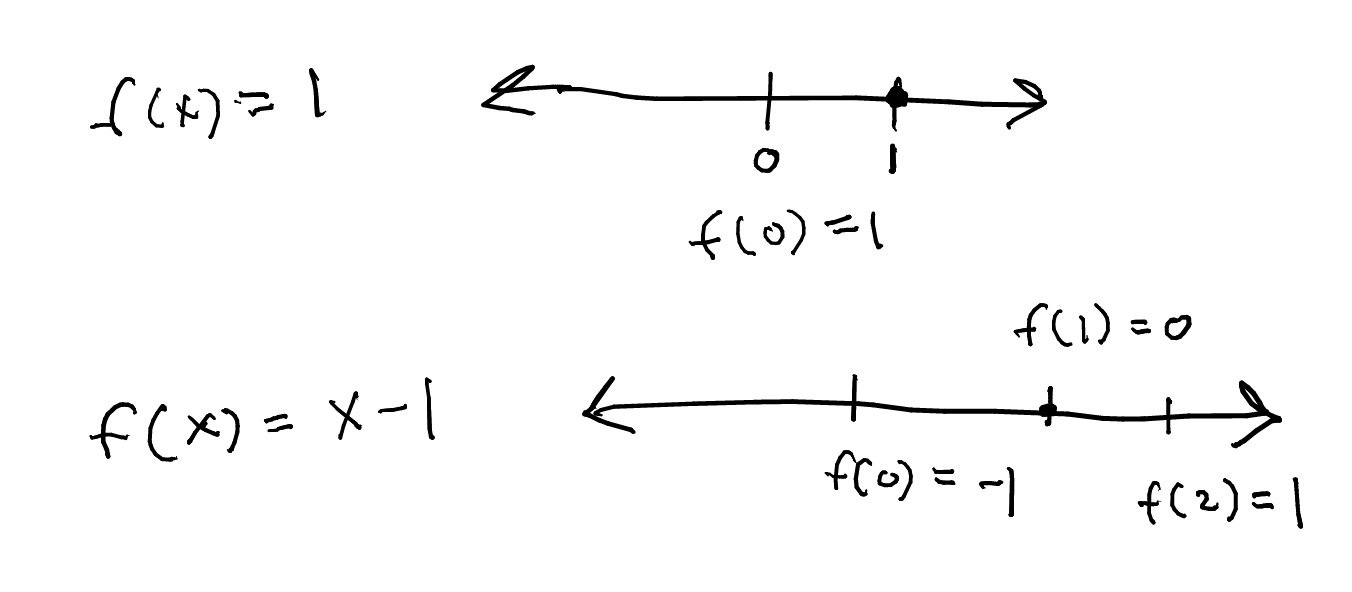
\includegraphics[width=0.75\textwidth]{img/implicit_sketch.png}
  \caption{Number line illustrating the construction of an implicit signed function}
  \label{fig:implicit-sketch}
\end{figure}

Researchers at MIT have taken these principles to constrain
geometric features to ensure a part can be manufactured.\cite{Shugrina_Shamir_Matusik_2015}
They call their system ``FabForms" and shows how functional representations
can easily accept constraints.

More importantly, functional representations can naturally deal with affine
transforms. \cite{Henderson_2002} Given some transform associated with a
FRep, one simply applies the inverse transform to check membership.

\section{Logical operations on Distance Fields}


One can also compose functional representations with set operations. 
Below are basic set operations defined for these functions:

\begin{equation*}
\cap : \mathtt{min}(f_1,f_2) \\
\end{equation*}
\begin{equation*}
\cup : \mathtt{max}(f_1,f_2) \\
\end{equation*}
\begin{equation*}
\neg : -\mathtt{f}_1
\end{equation*}

It follows that the ``difference"
of $f_1$ and $f_2$ is the intersection of $f_1$ with the negation of $f_2$,
$\mathtt{max}(f_1,-f_2)$.
The mathematical analyst might have trouble with these formulations because
such operations
create discontinuities.


\subsection{Rvachev Functions}

In the 1960's Vladimir Rvachev produced a method for handling the "inverse
problem of analytic geometry". His theory consists of functions which provide a
link between logical and set operations in geometric modeling and analytic
geometry.\cite{shapiro1991theory} While attempting to solve boundary value problems,
Rvachev formulated an equation of a square as
\begin{equation*}
a^2 + b^2 − x^2 − y^2 + \sqrt[]{( a^2 − x^2 )^2 +( b^2 − y^2 )^2} =0
\end{equation*}

Implicitly, the sides of a square can be defined as $x= +/- a$ and $y= +/- b$.
The union of these two is a square. By reducing the formulation of the square
we can generalize an expression for the union between two functions.
\begin{equation*}
\cup : f_1 + f_2 + \sqrt[]{f_1^2 +f_2^2} =0
\end{equation*}

Likewise we can see that intersections and negations can be formed for logical
completion.
\begin{equation*}
\cap : f_1 + f_2 - \sqrt[]{f_1^2 +f_2^2} =0 \\
\end{equation*}
\begin{equation*}
\neg : -f_1
\end{equation*}

These formulations can be modified for $C^m$ continuity for any $m$.
\todo{show this construction, it isn't obvious}
\cite{shapiro2007semi} In addition Pasko, et. al. have shown that Rvachev
functions can serve to replace a geometry kernel by creating logical
predicates. \cite{pasko1995function} Their research also establishes the
grounds for user interfaces and environment description. For this work a
practical implementation will most likely leverage their insights.
Rvachev and Shapiro have also shown that using the POLE-PLAST and SAGE
systems a user can generate complex semi-analytic geometry
as well.\cite{rvachev2000completeness} 

While a functional representation for geometry is mathematically enticing on
its own, the power it gives for numerical analysis might be its greatest
virtue. Numerical analysis justified the initial investigation by Rvachev
early on. A boundary value problem on a R-Function-predicate domain allows
for analysis without construction of a discrete mesh.\cite{rvachev2000completeness}

One of the most general expositions in the English language of R-Functions
applied to BVPs is
Vadim Shapiro's``Semi-Analytic Geometry with R-Functions". \cite{shapiro2007semi}
Unfortunately, no monographs about R-Functions exist in the English literature.
Most literature is in Russian, however many articles presenting applied
problems using the R-Function Method. \cite{voron2010}

Such a system for analytic geometry can be developed further. In the context
of an Eulerian flow field, a distance field over a function that
generates partial derivatives could be a fast numerical computation method.


\subsection{Signed Distance Fields}

\todo{rewrite to be salient}

A signed distance field (SDF) is a uniform sampling of an implicit function,
or any oriented geometry. \todo{didn't introduce orientation, winding order, etc...}
Below
we can see this in action over the definition of a circle.

\begin{lstlisting}
julia> f(x,y) = sqrt(x^2+y^2) - 1
f (generic function with 1 method)

julia> v = Array{Float64,2}(5,5) # construct a 2D 5x5 array of Float64

julia> for x = 0:4, y = 0:4
           v[x+1,y+1] = f(x,y)
       end

julia> v
5x5 Array{Float64,2}:
 -1.0  0.0       1.0      2.0      3.0    
  0.0  0.414214  1.23607  2.16228  3.12311
  1.0  1.23607   1.82843  2.60555  3.47214
  2.0  2.16228   2.60555  3.24264  4.0    
  3.0  3.12311   3.47214  4.0      4.65685
\end{lstlisting}

The results of \texttt{v} might be confusing since the matrix is oriented with
the origin in the top left corner. At coordinate $(0,0)$, or entry \texttt{v[1,1]},
we see that \texttt{f} is
equal to \texttt{-1}. Likewise we can see $(0,1)$ and $(1,0)$ are points on
the boundary since the value is \texttt{0} and everywhere else is positive.

Distance fields are interesting since they provide an intermediate representation
between functional space and discrete-geometric space. However they are
a very memory hungry data structure. Pixar has published OpenVDB which helps
work around these concerns, but such compression can be lossy.\cite{OpenVDB}
With the advent of shader pipelines for GPUs, distance fields have become
more popular. Valve has used SDFs with great success for generating smooth
text.text renders. \cite{Green_2007}
Many algorithms for generating polyhedra from an SDF
exist. The most common are Marching Tetrahedra, Marching Cubes,
and Dual Contours.\cite{Muller_Wehle_1997}\cite{Newman_Yi_2006}\cite{Cook_Hourvitz}

\todo{Talk about vert and frag shaders.}

Andreas Bærentzen and Henrik Aanæs published methods on the inverse
problem of converting a mesh to a signed distance fields.\cite{Baerentzen_Aanaes}
DiFi was introduced in 2004, which demonstrates an algorithm for creating
SDFs on multiple types of geometry \cite{Sud_Otaduy_Manocha_2004}.
\todo{Need to re-read this paper}

Many necessary algorithms in path planning for digital manufacturing tools
fall out of distance fields. For example, offsetting simply becomes
an addition or subtraction over the SDF. Computing the medial axis becomes
a scan for inflection points. Many path planners need to simplify polygon
representations as to not generate move less than the resolution of the machine.
Assuming the machine uses a Cartesian system, a SDF can correspond perfectly
to the lowest available resolution of the machine.
Likewise as Stereolithographic 3D printers
begin to use digital mirror devices (commonly known as DLP or DMD)
, discrete representations of geometry will become more important in
digital manufacturing.

\cite{Pasko_Adzhiev_Comninos_2008}

\section{Simplices}

Recently a Simplex type was added to GeometryTypes. A Simplex is defined
as the minimum convex set containing the specified points. The initial
prototype is very simple yet works well. Below we can see a 0th and 1st order
simplex constructed in $\mathbb{R}2$ and $\mathbb{R}3$
\begin{lstlisting}
julia> using GeometryTypes

julia> Simplex(Point(1,2))
GeometryTypes.Simplex{1,FixedSizeArrays.Point{2,Int64}}((FixedSizeArrays.Point{2,Int64}((1,2)),))

julia> Simplex(Point(1,2,3), Point(4,5,6))
GeometryTypes.Simplex{2,FixedSizeArrays.Point{3,Int64}}((FixedSizeArrays.Point{3,Int64}((1,2,3)),FixedSizeArrays.Point{3,Int64}((4,5,6))))
\end{lstlisting}

This representation makes it possible to write code based on the order and
dimensionality of a simplex. Few algorithms have been developed around the
new Simplex type, and unfortunately it is not integrated as a lower-level
construct for the other types yet.

In addition I would like to add a Simplical Complex type.\footnote{\url{https://en.wikipedia.org/wiki/Simplicial_complex}}


\section{Polytope}

\subsection{Descrete Form}


\subsection{Continuous Form}
